\documentclass[a4paper,10pt]{article} 
\usepackage[margin=3.2cm]{geometry}
\usepackage{booktabs} 
\usepackage{graphicx} 
\usepackage{amssymb}
\usepackage{amsmath} 
\usepackage{xcolor}
\usepackage{setspace} 
\usepackage{natbib}
\usepackage{hyperref}
\usepackage{doi}
\usepackage{pdfpages}
 
\onehalfspacing

\newcommand{\revpoint}[3] 
{ \hrule ~\\[0.5em]
\noindent\textcolor{gray}{\noindent#1} \\[0.5em]  
\noindent\textcolor{blue}{\textit{\noindent#2}} \\[0.5em]
\noindent\textcolor{black}{\noindent{#3}} \\[0.5em]
}

\newcommand{\com}[1]{\textcolor{red}{\noindent#1}}


\title{Response to Reviewers} 
\author{Cedrick Ansorge and Hauke Wurps }
\begin{document}
\maketitle

%-------------------------------------------------------------------------------------%

%######################################################################################%
% not all comments are included, only where action is needed.
%######################################################################################%

\section*{Response to Reviewer 1}

Dear Reviewer 1, \\[1em]

\noindent Many thanks for the positive feedback on our manuscript. We have addressed the minor points raised in your review and hope that you agree with the edits. Pleas find the detailed responses below.  \\[1em]


\noindent Kind regards, \\[0.5em]

\noindent Cedrick Ansorge and Hauke Wurps  \\[0.5em]
%-------------------------------------------------------------------------------------%


\revpoint{The authors analyze wind speed and direction profiles in turbulent Ekman flow using asymptotic theory and DNS data. They found that the streamwise velocity follows classical scaling laws, while outer-layer profiles align with a modified Ekman spiral. They showed that the spanwise component exhibits mixed scaling near the surface and outer scaling farther out. \newline  Overall, the analysis and DNS are conducted rigorously, providing valuable insights and contributing meaningfully to advancements in the field.}{We sincerely thank you for the positive assessment of our manuscript and the appreciation of our work.}{}

\revpoint{In line 47, friction velocity is denoted as $u_* = \sqrt{|\tau_{sfc}/\rho}$. However, in Eq. (1a) (below line 179), $\tau_{sfc}$ is defined as the kinematic shear stress. Please make them consistent. }{Manz thanks for spotting this inconsistency in nomenclature. We have aligned $\tau_\text{sfc}$ with the conventional definition of dynamic shear stress and now include the division bz density in Eq. (1b).}{\begin{subequations}\begin{equation}
    \underline{\tau}_\mathrm{sfc} = \left(\begin{array}{c} \tau_x\\ \tau_y\\\tau_z\end{array}\right) = - \rho\nu \left( \frac{\partial U}{\partial z} \hat{e}_x + \frac{\partial V}{\partial z} \hat{e}_y\right)
  \end{equation}
  and labelled by an upper index $\alpha$ as in $\underline{U}^\alpha$ for the velocity vector, and
  (ii) the coordinate system aligned with the free-atmosphere geostrophic wind labelled by an upper index $G$ as in $\underline{U}^G$.
  %
  We denote the square root of the modulus of surface shear, the surface friction, by
  \begin{equation}
    u_\star = \sqrt{ \frac{|| - \underline{\tau}_\mathrm{sfc} ||}{\rho} } 
    \label{eqn:ustar_def}
  \end{equation} and let $Z_\star=G/u_\star$;
\end{subequations}}

\revpoint{Location for the definition of $z^-$. The first appearance of $z^-$ is at line 262, and figure 1b, but it was defined on line 307. It would be better to define it close to where it appears. }{Thank you - we now introduce the outer length scale much earlier in Sec. 2.1 ("Notation and governing equations"). We also think, this is more appropriate.}{The outer normalization (with respect to the boundary-layer depth $\delta$ and velocity $u_\star$) is denoted 
by a superscript $'-'$, i.e. $z^-=z/\delta$.  }

\revpoint{Figure 4: Should the legend be $Z_* = 4 log(Re_D) -8$, instead of $u_\star* = ...$"?}{Indeed, there was a typo, please find the revised Figure below.}{
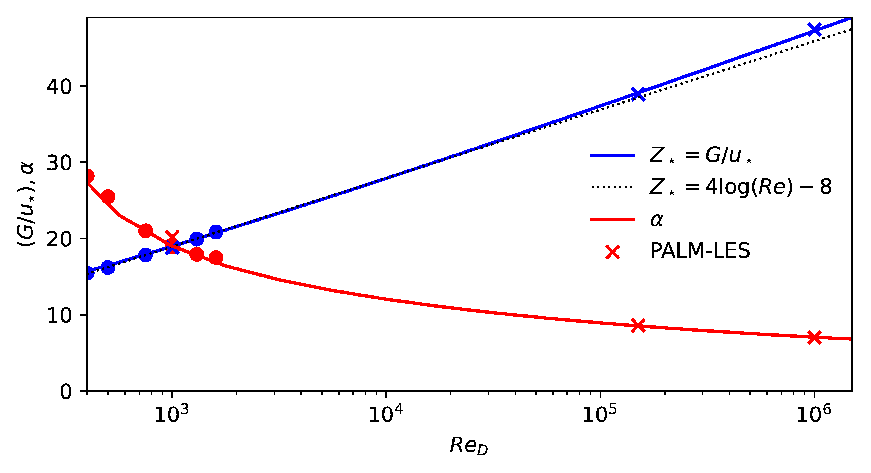
\includegraphics[width=\textwidth]{Fig4.eps}
}
\newpage
\section*{Response to Reviewer 2}
\revpoint{The authors perform direct numerical simulations of the Ekman layer at moderate Reynolds number, and use their simulations to examine the vertical mean velocity profiles in rotating, neutrally-stratified flows that serve as a proxy for the neutral atmospheric boundary layer. They compare their DNS results to a model that matches the Ekman model (in the outer layer) with the classical results for the inner layer (viscous layer plus log layer) in wall-bounded turbulent flows. Specifically, they examine the scaling of the spanwise velocity profile, and find that a matching procedure—combining both inner- and outer-scaling—is necessary. The article is generally clear and well-written, and addresses the important problem of how velocity profiles behave in the Ekman layer. Despite being an old problem, it has not been resolved, and there are many subtleties that are often neglected in the literature. I am overall supportive of this manuscript, but below I provide some specific comments which I believe will help improve the clarity of communication in the article. I am recommending that the manuscript is accepted in BLM, pending minor revisions. }{}{}

\revpoint{L. 12, 76: discussion of span-wise velocity component. Can you explain how you are defining streamwise and spanwise here? Are you assuming the streamwise component is aligned with the geostrophic wind direction far above the surface? }{}{}
\revpoint{L. 16 outer height - do you mean outer length scale? }{}{}
\revpoint{L. 19 “vide Reynolds numbers” - I’m not sure this makes sense to me. }{}{}
\revpoint{L. 63 Prandtl-layer height is undefined here}{}{}
\revpoint{L. 124 - “require one to consider” or “require consideration of” }{}{}
\revpoint{ll. 168-170 - This seems to be contradictory. The authors state that rotation only acts on the horizontal components of velocity, but go on to state that they neglect rotational effects on the horizontal components of velocity. }{}{}
\revpoint{l. 176 - I do not think that Ensemble should be capitalized }{}{}
\revpoint{L. 193 “this state is defined by a Reynolds number, the only non-dimensional parameter that governs the system.” Shouldn’t the Rossby number also enter as a non-dimensional parameter? Given a domain height, geostrophic wind speed G, and Coriolis parameter f, one can also define the Rossby number. The problem would depend on Reynolds number alone in the absence of rotation, but if there is rotation, the relevant dimensionless parameters should be both Re and Ro. }{}{}
\revpoint{L. 221 - It might be better to use scientific notation here. }{}{}
\revpoint{L. 277, 281 - the notation is a bit awkward here, e.g. $V^{\alpha_* +}(z^+)$. Is there a way to make it clearer? }{}{}
\revpoint{Fig. 1a - Does the solid black line correspond to the Re=1600 case? If so, why is there i a discontinuity just above $10^1$? Or are you also using a solid black line to denote the inner layer velocity profile, $u^+ = z^+$? }{}{}
\revpoint{L. 308 Eddy should not be capitalized}{}{}
\revpoint{L. 311 - The assumptions of horizontal homogeneity and W=0 are not exactly the same thing as symmetries in the flow. }{}{}
\revpoint{Fig. 3: It would be better to present heights in terms of z+ values rather than the index of the vertical coordinate. }{}{} 


\newpage
\section*{Response to Reviewer 3}
\revpoint{This is an excellent paper that should be published in BLM. However, I request the authors to tone
down their narrative, including the title. It is an empirical study that tries to fit DNS data using various
formulations. Some of these formulations have a physical basis, while others are ad-hoc. Please refrain
from calling the results “universal”. } {}{}

\revpoint{At the heart of this paper is Eq.~10a. Following Etling's work and others, this equation has been derived in Appendix A1. \newline 
  \[
    \frac{1}{G} \left(\begin{array}{c}U_\text{Ek} \\ V_\text{Ek} \end{array}\right) = \left(\begin{array}{c} 1 \\0 \end{array}\right) + e^{-z_\text{Ek}} \left[ a_\text{ek} \left(\begin{array}{c} -\cos z_\text{ek} \\ \sin z_\text{ek} \end{array}\right)+ b_\text{ek}\left(\begin{array}{c}\sin z_\text{ek} \\ \cos z_\text{ek}\end{array}\right)   \right]
  \] \newline  
  The problem with this equation is the assumption of constant eddy viscosity. As the authors showed in
  Figure 2c, the eddy viscosity profile from the DNS is far from constant. It has a clear maximum and a
  specific shape, which depends on Re.
  So, the authors took an empirical (engineering) approach on page 14 (line 403). They estimated a bulk
  eddy viscosity indirectly. This is a major weakness of this paper and could be avoided. Please see the
  following paper where we analytically derived the eddy viscosity profile from the Ekman equations.
  Since this is a relatively new paper, the authors might not have come across it. That is why I am revealing
  my identity.
  \begin{quotation}Basu, Sukanta, and Albert AM Holtslag. “A novel approach for deriving the stable
  boundary layer height and eddy viscosity profiles from the Ekman
  equations.” Boundary-Layer Meteorology 187.1 (2023): 105-115.
  \end{quotation}
  The authors might want to revise their derivations based on our analytical eddy viscosity profile. If that
  is difficult to do, I suggest highlighting the limitations of their current bulk approach. Also, emphasize
  the limitations of Eq. (10a) as it assumes constant eddy viscosity. }{}{}

\revpoint{Could the authors comment on Fig. 6a in the revised manuscript? The discrepancy between DNS and
  their empirical prediction is large and not explained.
}{}{}
\end{document} 